\chapter{Story Lane Theater 2}

% \begin{figure}[H]
%     \centering
%     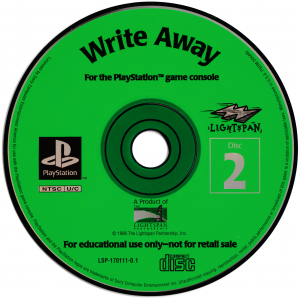
\includegraphics[width=\textwidth/2]{./Games/WriteAway/Images/WriteAway2CD.jpg}
%     \caption{Write Away 2 CD}
% \end{figure}

The second of the Story Lane Theatre games published and released by The Lightspan Partnership for the PlayStation 1.

Story Lane Theatre 2 features two video programs:

\begin{itemize}
    \item Finn McCoul
    \item John Henry
\end{itemize}

\clearpage
\newpage

\section{Finn McCoul}

\subsection{Audio Summary}

Fionn mac Cumhaill is the hilarious legend in which the famous Irish hero and his clever wife Una defeat the brutish giant Cú Chulainn once and for all. The story is told by Catherine O'Hara, and the music is by The Boys of the Lough. Backstage Pass visits with the musicians Cathal McConnell and Dave Richardson from The Boys of the Lough.

\subsection{Transcription}

Come on in, settle back. It's curtain time at the Story Lane Theater. You've never seen a stage like this one. Anything can happen here.

Today we're going to watch the story of Fionn mac Cumhaill, Ireland's most famous giant. We'll visit Fionn's home on Knockmany Hill and watch as Fionn and his wife Una prepare to do battle with the powerful and terrifying giant Cú Chulainn. But before we see the story, let's share a few moments with two of the musicians who perform the music you'll be hearing in the show. The man playing the tin whistle is an Irish musician named Cathl McConnell, and the man playing the accordion is Dave Richardson, who comes from England. They both travel all over the world performing with a group called The Boys of the Lough. Let's hear Cathal and Dave tell us more about their music.

"Got my musical interest from my father, no doubt about that. My father was called Sandy McConnell. He was a good singer, he played the whistle, and in his younger days, he played the accordion. When my father got me a little tin whistle for Christmas, it seemed that the whistle was the right instrument for me to play."

"If you look at music in any culture, music is a way of communication. It's a way of expressing ideas or emotions, and lots of people like to listen to music because it reflects things that they feel or things that they think. If we look at Irish music as we see it now or as we hear it, it's been handed down for hundreds of years and it's still in very good condition. I think this is because people in Ireland continue to live, many of them in the country, and the old ways survive, the old ways of meeting with one another and talking to one another, playing music together."

"I first heard the story of Fionn mac Cumhaill from my mother. It's a dramatic sort of story. It's a story of the impending battle of the two giants. It's a bit of a challenge to put music to a story because you really have to think about it."

"We tried to decide what kind of music would fit these characters to support the story that was being told. We think about the bad guy Cú Chulainn, and we think of dark, heavy, sinister music for him. And we thought of maybe using very low notes on the instruments. We used a little instrument called an accordion and used the bass on it. He looks dark, menacing. You wouldn't want him coming to your birthday party. He's the guy who'd steal all the cookies. For Fionn, we wanted something a bit more light and comical. He looks like he'd be a lot of fun and at the same time, he doesn't look too street smart. I think he misses one or two things in life. So we decided to use lighter instruments like the tin whistle. The wife of Fionn, Una, is a very good friend to Fionn. She's his best friend. That's why he married her. She's a very busy woman, active, happy. She's very content. So we chose light instruments and very light rhythms like the jig and the polka. This business of writing tunes is unusual. You don't have to take out a pen and paper and write them. You sit with an instrument in your hand and your fingers on the instrument, and you move your fingers around, and suddenly a little piece of melody catches your ear and you think, "I like that." That's the start of an idea. And then it might all click together, you know.It's just like making up a little poem or something."

"Playing this music gives a lot of pleasure to a lot of people. As time goes on, it's being played more and more. There are an awful lot of young people learning this music now, much more so than when I was young."

"It's very interesting to think about what we get from music as people. I think it reminds us of how much like other people we are. They can be people in other countries in the world, or they can be people who lived in the past. They can play you a tune or sing you a song, let you hear a melody, and you know that they're the same kind of person as you."

And now here come the sounds and sights of Fionn mac Cumhaill.

Fionn mac Cumhaill was the most famous champion Ireland ever knew. Fionn was a giant to be sure, but when he was born, he was no bigger than a fire-breathing dragon. And as giants went in those days, that was a might on the wee side. Now King Cumhaill was Fionn's father, and being a famous Irish giant himself, he took the lad's small size to heart.

"I have a boil on me flank that's bigger than he is," said King Cool on seeing the boy for the first time.

King Cumhaill was so distraught over Fionn's size that he took the child to the castle parapet, wiped the potato-sized tears from his eyes, and gently punted him into the loch below. Now the grandmother of the lad, King Cumhaill's mother, just happened to be on the shore watching as the infant plunged into the water.

"Why that's me own flesh and blood splashing about there," she said and immediately dove in.

In two shakes of a lamb's tail, she dragged the child out of the loch and rushed away with him deep into the woods.

Finding a nice stout tree, the grand dame took out her hatchet and chopped a chamber within it, and there the two of them lived. For years, the old woman lovingly fed Fionn a diet of tree bark, peat, and the occasional grub, but the child thrived nonetheless. After some time, the boy rather outgrew his surroundings, and it was then that his grandmother knew it was time to send him out into the wild and cruel world.

Now such an inauspicious beginning to a life has been known to spoil a man's disposition entirely, but not young Fionn. He thanked his grandmother for looking after him, kissed her gently upon the head, and set out to distinguish himself as a great hero. Why, he was as strong as two dozen oxen and as swift as 43 hares, and he trod all over the emerald countryside, taking a glen at a step, a hill at a leap, and locks at a bound.

Before too long, Fionn took a wife for himself, and her name was Una. Una was a beauty, as they say, and a giant as herself. Aye, and that sun-kissed lass was a clever one too. They were a matched pair, they were, with Fionn's brawn and Una's brain. Together they lived quite happily upon the top of Knockmany Hill in Ulster. People always wondered why it was that Fionn had selected such a windy spot for his dwelling.

Now Fionn made his share of excuses for choosing to live in the middle of nowhere, but the real reason Fionn made his home atop Knockmany was to see Cú Chulainn coming.

"Oh, Cú Chulainn! It sends shivers down me spine to even utter the name. Cú Chulainn\dots"

No other giant in all of Ireland could stand before him. It was said, and I personally know for a fact 'tis true, that by a single blow of his fist, he once flattened a thunderbolt into the shape of a pancake. He always carried it about with him in his pocket, and before he got into a fight with one of his foes, Cú Chulainn would show them the pancake just to give them a notion of the kind of pulpin' they're about to receive.

Cú Chulainn had given every giant in Éire a considerable taring, every one of course but Fionn himself. But that was only own to the fact that whenever Cú Chulainn went after Fionn, our hero would run in the opposite direction. Now at this time, Fionn was buildin' the causeway from Ireland to Scotland. It was a grand undertaking even for Fionn, so he had his band of champions called the Fenians assistin' him.

One day down at the causeway, Fionn and his men were rearranging the coast and moving a few small cliffs when he began gnawnin' upon his thumb. You see, this is how Fionn called upon his singular gift for prophecy. Whenever he got into a fix and he couldn't fathom the choices that life so often presents, he would suck his thumb for inspiration, and a most curious thing would occur. He would see the future before him as clear as day, for it was in his thumb that his power for prophecy resided.

Now at that precise moment, Fionn had divined from his thumb that Cú Chulainn was coming to the causeway to do battle with him. And it was just then that Fionn discovered a very warm and sudden fit of affection for his wife.

"I need to see me love Uma," said Fionn. "Me thumb tells me so. Me thinks she's in danger."

"But Fionn," pleaded Conan the Bald, one of the Fenians, "what about the causeway?"

Alas, it was no use. Fionn was already well on his way to Knockmany.

"God save all here," said Fionn.

"Musha, Fionn," said his wife, "welcome home to your own Una, you darling bully. And what brought you home so soon Fionn?"

"Why me sweet rose, nothing but the purest of love and affection for ye, of course." After Fionn spoke, he clapped his thumb into his mouth.

"Fionn sweetness," said Una, "please don't do that while you're talking to me. It's not polite."

"He's a-coming," said Fionn. "I see him below [Dan Ganon]."

"Who's coming?" said Una. "Who are you talking about?"

"It's that nasty Cú Chulainn, it is. Oh, it's said that when he gets angry and begins to stamp, a dozen earthquakes erupt. And when he does battle with thunderbolts, he flattens them into tiny pancakes and then eats them with honey, a whole hive of it, and with the bees still buzzing inside it."

"Gracious, the brute!" said Una.

"I don't know how I'll manage. If I run away again, I'll be disgraced before me people. And my thumb tells me that I must meet him sooner or later."

"Well, my bully, don't be downcast," said Una. "Leave it to me and I'll bring you out of this scrape better than you might on your own."

Now it so happened that Una had a sister named Granua who lived upon a hill called Kylemore, just opposite Knockmany. The beautiful valley that separated the two sisters was only four miles wide, and so on a summer's evening when they wanted to talk, Una and Granua only had to put their heads out the windows of their homes.

"Granua, are you home?" said Una.

"I am, sister dear," said Granua. "And how have you been today?"

"Well, not so well, I'm afraid," said Una. "Would you do us the favor of looking about from your window and telling us what you see?"

"Well, nothing, sister dear. Tis only a mountain coming over this way," said Granua. "Nothing to trouble yourselves over."

"A mountain? That's no mountain," said Una. "That's the giant Cú Chulainn, and he's coming to leather our Fionn. Perhaps if you delay the brute, it'll give me a moment to think. Why don't you ask him up for a bite?"

"I only have 50 pounds of butter, that's not nearly enough to make a cake for that giant," said Granua. "If you toss me over a ton or two, you'll oblige me very much."

So Una got the largest tub of butter she had and called up to her sister, "Granua, are you ready?" said Una. "I'm going to throw now."

Una gave the butter a mighty heave, but in her anxiety over Cú Chulainn, she forgot to say the magic words that were to make it fly to Granua. And so the butter landed with a thud halfway between the two hills.

"My curse upon you, baleful butter!" cried Una. "You've disgraced me!"

And with that said, the butter turned instantly to stone. It lies there today, exactly as it came out of Una's hand, with a mark of her four fingers and thumb imprinted upon it.

"Oh, never mind," said Granua. "I'll do the best I can to stall Cú Chulainn."

So Granua baked her cake anyway and signaled Cú Chulainn to come up to Kylemore. She placed the cake before the giant, and without so much as a "thank ye miss," Cullin threw it into his mouth and devoured it in one frightening bite.

"Needs butter," he grunted, licking the last crumbs from his fingers, and proceeded on his way.

In the meantime, Fionn was in quite a panic on Knockmany.

"Una, can you do nothing for me? Where's all your invention, woman? Will I be skivered like a rabbit before your eyes and have me name disgraced forever before all of Ireland? How can I fight a man who scares the fire out of thunderbolts?"

"There now, be easy, Fionn," replied Una. "I've got an idea. Just leave it to me."

With that, Una went to work. First, she rummed about and found 21 iron griddles. Then she took the griddles and kneaded them into the middle of six loaves of bread. She then baked the loaves on the fire, setting them aside in the cupboard when they were done. Finally, Una took a large pot of new milk, which she made into curds and whey, and then whispered something into Fionn's ear.

And just as Cú Chulainn was coming across the valley, Una fetched a baby's cradle and instructed Fionn to lie down in it. "Say nothing and follow me lead."

"I will, but I don't like it one bit."

Just as he was getting settled, Cú Chulainn burst through the door. "Be this the home of the great Fionn mac Cumhaill?" he asked.

"Aye, it is indeed," said Una, "but he's not in at the moment. Someone told him that a big bassoon of a giant called Cú Chulainn was down at the causeway looking for him, so he rushed away to catch him. Can I help ye?"

"I am Cú Chulainn," said he, looking puzzled. "And I've been after your husband for 12 months."

Una let out a loud, mocking laugh and looked at him as if he was only a little pip of a man. "If you take my advice, you poor looking creature, you'll pray day and night that you may never see him," said Una. "It'll be a black day for you if you do."

"Ha!" Cú Chulainn snorted, dismissing Una's warning.

"Ah now, the wind's blown against the door," said Una. "Seein' as how Fionn is away from home, would you be civil enough to turn the house around?"

Now this request took Cú Chulainn back, for even he didn't do this sort of task on a daily basis. Nevertheless, he pulled the little finger of his right hand three times and went outside. He then put his massive arms about the house and, with some effort, turned it in a position favorable to the wind.

"Thank ye kindly," said Una. "Please stay and have a bit of me humble fare. Even though you and Fionn are enemies, he would scorn me if I didn't treat you kindly in his own home."

Una brought Cú Chulainn to the table and placed before him the half dozen loaves of bread she had baked, together with 10 sides of bacon and a stack of steaming cabbage. Cú Chulainn greedily stuffed one of the loaves into his mouth and took a tremendous bite. When Cú Chulainn's teeth struck the griddle that lay in the middle of the loaf, the entire house shook.

"Oh, blood and fury!" shouted Cullin. "And just what sort of bread is this you've given me, I might ask?"

"What's the matter?" said Una.

"Matter?" shouted Cullin. "Why, what's the matter indeed? Here the two best teeth in me head smashed to smithereens!"

"Oh, it's a pity that I forgot to tell you that nobody but Fionn himself can eat it, and his little 'un who sleeps in the cradle over there."

"Take your bread away, I'll not have another tooth in my head."

"Now, now," said Una, "don't be waking the child with all your bellyaching."

Then Fionn gave a shriek that startled the giant.

"Now you've gone and done it. You've awakened him," said Una.

"Maa," said he, "I'm hungry and I want something to eat."

Una went to the cradle and gave Fionn one of the loaves of bread that had no griddle in it. After a few bites, he realized it was safe and made the rest of the loaf disappear in two bites.

Cú Chulainn was thunderstruck, and by the look on his face, Una knew her plan was working.

"I'd like to have a look at the lad in the cradle," said Cú Chulainn. "Any child who can manage that bread is in good fighting trim."

"Get up and say hello to our guest, [Milam]," said Una, motioning to Fionn. "It's terribly shy when company comes. Not many travelers get up our way, you know."

Fionn crawled out of the cradle and toddled over to Cú Chulainn.

"Are you strong as me, da?"

"What a boom voice and such a young babe."

"Just a touch of the whooping cough," Una explained with a smile.

Then Fionn grabbed a white stone and handed it to Cú Chulainn. "Can you squeeze water out of this white stone?" said Fionn.

Cú Chulainn was puzzled, but as he intended to humor the lad, he took the stone and squeezed it as hard as he could, but it was no use. He might be able to turn the house around or flatten a thunderbolt into a pancake, but squeezing water out of a rock was something else entirely.

"You call yourself a giant? Me da can do it, and he showed me how. Give me that stone."

Fionn took the stone from Cú Chulainn and then slightly exchanged it with the curds, just as Una had instructed, and he then squeezed the curds until the whey squirted out in a little shower from his hand, clear as water.

"I don't care to waste my time with a giant the likes of you. You'd better be out of here before me da comes back, or else he'll make porridge of you and serve you for dinner."

Now Cú Chulainn was taken quite aback. "He's a lucky man to be sure, to have such a handsome wife and a son who snacks on iron and squeezes water from dry stones. I see I have misjudged him terribly. If it's all the same to ye, I think I'll stay a bit for Fionn's return. It would do me proud to make the acquaintance of a great hero such as he, and I shall have to apologize for chasing him hither and yonder for all these months. Yes, apologize I must, even if it takes Fionn a fortnight to return."

With that, Cú Chulainn sat next to Fionn's cradle and rocked it somewhat roughly, as giants will do, and hummed a soothing giant lullaby. Poor Fionn saw his very life pass before his eyes.

"Oh, me bones!"

"What is wrong with the child?" asked Cú Chulainn.

"Um, uh, the poor lad is teething," said Una. "His gums have been smarting lately. There's nothing that can be done."

"I'm not so sure of that," said Cú Chulainn. "Me own dear mother had a little trick she used when me choppers come up." With that, Cú Chulainn reached for the flask of spirits he kept in his hip pocket. He poured a touch upon the little finger of his right hand and opened Fionn's mouth with his left. Then he massaged Fionn's gums with a spirit-soaked finger. "The spirits will dull the boy's pain," said he.

Now it was bad enough to have Cú Chulainn in one's house, but to sit back and take his little finger in the mouth was unpardonable. "Now just a little bit more, laddie. Aaah," said Cú Chulainn as he lovingly administered another dose. "You know, Mrs. mac Cumhaill, I think after I've made your husband's acquaintance, I will take a wife so that I may have a son just like yours."

"It's the teeth way in the back of his mouth that are the worst," said Una. "You're such a help, kind man." And at that moment, Una decided to take matters into her own hands. She grabbed the pot that hung in the hearth and, rearing back, she hurled it at the head of the giant with all her might. Instead of Cú Chulainn, however, the pot struck poor Fionn dead upon the crown. The concussion was so great that Fionn clamped down upon Cú Chulainn's little finger, which was still applying the spirits, lopping it off at the third knuckle.

"Aah! Look what the boy has done to me!" Cú Chulainn groaned, holding his maimed right hand. "I'm finished!"

You see, the giant's huge strength all lay in the very little finger of his right hand, which Fionn had 'accidentally' separated from its master. Cú Chulainn then let loose with another ear-shattering scream. Then right before the eyes of Fionn and Una, he shrunk from the size of a giant to that of a timid little church mouse.

Now Una and Fionn had a large tom cat who liked to sleep behind the stove, but all the commotion woke him, and when he came out to investigate, there stood the oddest looking mouse he had ever seen. Without much ado, the tom cat chased the screaming former giant down Knockmany, around the locks, and across the fields right into the sea.

"Glory be!" said Fionn in triumph. "There isn't a giant in all of Éire as great as myself. I have defeated the great Cú Chulainn!" Una picked up her newly dented pot and gazed meaningfully into her dear husband's eyes. "Uh, or perhaps should I say we have defeated the great Cú Chulainn?"

And truer words were never spoken.

\subsection{Credits}

Told by: Catherine O'Hara;
Illustrator: Peter de Sève;
Written by: Brian Gleeson;
Music Composed by: Boys of the Lough;
Music Performed by: Aly Bain (fiddle), Cathal McConnel (flutes), David Richardson (concertina + mandoline + cittern + accordian), Christy O'Leary (uillean pipes + accordian + whistle), John Coakley (piano + guitar + fiddle), Jim Sutherland (bodhran + percussion);
Music Produced by: Jim Sutherland, Boys of the Lough;
Music Recorded and Mixed by: Daniel Protheroe, Jim Sutherland;
Music Coordinator: John Ullman;
Soundtrack Mixed by: Chris Nelson;
Editor/Animation Camera: Mark Forker;
Assistant Editor: Stephen Marlin;
Post Production: Rebo High Definition Studio (New York NY);
Editorial Director: Eric Metaxas;
Art Director: Paul Elliott;
Associate Producer: Doris Wilhousky;
Producer: Ken Hoin;
Director: C.W. Rogers;
Executive Producers: Mike Pogue, Mark Sottnick;

\section{John Henry}

\subsection{Audio Summary}

John Henry tells the legend of the mightiest dog gone nation builder this country has ever seen, who single-handedly defeats the steam drill in a man-against-machine steel driving contest. The story is told by Denzel Washington, with much by B.B. King and Taj Mahal. Backstage Pass visits with blues musician Taj Mahal.

\subsection{Transcription}

Come on in, settle back. It's curtain time at the Story Lane Theater. You've never seen a stage like this one. Anything can happen here.

Today we're going to hear about a legend, the legend of John Henry. The story of this steel-drivin' man has been passed down mainly in a song. The song has been around for over a hundred years, and it changes a little every time someone new sings it, but it's always about a remarkably strong man and his race against a machine. We are going to hear two versions of that song today, performed in the style of music known as the blues, one from a musician named B.B. King, and the other from the man who's playing the music you're hearing right now, Taj Mahal. Taj has been playing the blues for practically his whole life. Let's hear what he has to say about his music and the legend of John Henry.

"The blues can express many moods and feelings, 360 degrees of emotion. Joy, sadness, fun, laughter, all kinds of things. It has the ability to take whatever life is and present it in a way that you hear it right away. There are some songs that came out of railroad work. That was a really hard job. You think about laying railroad track and tires, and that they used to do all that work by hand. That was all done by hand. Chanting rhythmically while you're doing that kind of work makes it go easier. The sun was hot, the work had to be done, and the freedom that they had was to rhythmically deal with this. That's something that they could do, so they sang their songs and the work goes much easier. The first time I heard the legend of John Henry, I cannot even recall. It was so long ago that I know it was before the age of five. That much I can tell you. But it came out of the folklore that was always being brought down the line, and that was one of the reasons why I wanted to play that song. It's a very important song."

"When John Henry was a baby boy, sitting on his daddy's knee, daddy said, 'Son, son, son, keep on looking to the sun. Don't you ever take no pattern after me. Don't you never take no pattern after me.'"

"John Henry actually takes an incident that happened out near Beckley, West Virginia, around the building of the Big Bend tunnel for the Chesapeake and Ohio Railroad. There was a race to see whether the man would hold up as good as the steam drill."

"John Henry said to the steam drill, 'Steam drill I'm gonna run you down. I'm hitting 9 pounds from my hips on down. Oh Lord, you go watch me throw down. Oh Lord, watch me throw down.'"

"John Henry is the struggle between humans and the machine. There's always the desire to show that the human touch is more important than the mechanical touch."

"John Henry hammered in the mountains, to the head of his hammer caught fire. 'I been pick them up, boys, won't you lay them down again? I want a cool drink of water 'fore I die, I want a cool drink of water 'fore I die, I wnat a cool drink of water 'fore I die.'"

"Legends started out because of people's desire to have hope. It usually is some sort of unique incident that happens, and then a lot of different people put their own little spin on it. In my opinion, what John Henry symbolized was endurance and strength to really come up against a formidable, a very formidable foe and triumph."

Thanks, Taj, for playing your version of the song. And now let's get ready to see the legend of John Henry. Be sure to listen for another version of the John Henry song by B.B. King, and you'll see how the legend of John Henry keeps right on growing all the time.

"Yeah, my name John Henry, and I'm a natural man. But I was born one morning with the hammer in my hand. And if one day I find myself out all alone, I'll hammer till the evening and found my way back home. And found my way back home, and found my way back home, and found my way back home."

Way back a good while ago, when the United States was still busting out of his baby shoes, there lived a man named John Henry. Now, ain't no history books going to tell you about John Henry 'cause he was just too plain big for them books. But when it comes right down to it, John Henry was the mightiest, doggone greatest nation-builder this country's ever seen. Oh sure, you had your Washingtons and your Jeffersons, but they was just Presidents. You see, John Henry was a steel-driving man.

Now some folks think they know all about John Henry and his famous race with the steam drill, but most of them don't even know a steel stake from a beef steak. See, I was around when John Henry was King of the railroad camps, and I remember him just as clear as the Kentucky moon on an August night. So y'all listen up, 'cause I'ma tell you the guaranteed, gold-plated, 99.9\% truth about John Henry.

Now it all started in a little village way down south in cotton country. Mama and Papa Henry were just your ordinary sharecropping folk, no different from the rest of us. They lived in a log cabin, and one springtime morning, Mama Henry gave birth to a baby named John Henry. Now folks knew right away there was something different about John Henry. Shoot, ain't no ordinary baby born with a hammer in his hand, and ain't no ordinary baby weighs over 45 lbs. But John Henry did, and that wasn't even the strange part.

Not two hours out of his mama's belly, John Henry ups and starts talking.

"Oh, if it ain't too much trouble," he said, just as sweet as sugar, "would y'all mind bringing me something to eat? I'm mighty hungry."

Now nobody ever heard a two-hour-old baby talking before, but after a while, Mama Henry asked John Henry what he wanted to eat.

"Well," he said, figuring and calculating on his fingers, "I'd like eight ham bones, uh, two pots of black-eyed peas, a three-foot slab of cornbread, three kettles of cabbage soup, a big heap of collard greens, four pans of peach cobbler, and, and two pots of coffee. Strong coffee. Uh, that is, if it ain't too much bother."

So John Henry ate pretty good, and he was so tuckered out when he was done, by jiminy, he slept for a solid week.

Well, the years went by, and John Henry grew bigger. At 2 years old, he was juggling chickens for fun. At 6, he was wrestling with razorback hogs and juggling chickens at the same time. And at 10, why, at 10, John Henry was already a teenager. But there was nothing in the whole wide world that John Henry liked more than swinging a hammer and singing a song. He'd hammer hickory sticks, he'd hammer fence posts, cooking pots, brass nails, boulders, anything he could get his hands on. He'd pound in the morning, clang in the evening. His arms grew as solid as oak stumps, and his chest busted out bigger than a barrel. Why, he grew so big that one day he couldn't even fit through the front door of his parents' cabin.

And that's when John Henry decided it was time to leave home.

"Mama," he said one morning, "I'm a man now. I'm a natural man, and I'm going to find me a job with a hammer in my hand."

So John Henry left home, and he walked north through the countryside. And as the sun went down at night, making the whole land light up like fire, he sang a song to himself.

"Yeah, my name's John Henry, and I'm a natural man. I was born one morning with the hammer in my hand. And if one day I find myself out all alone, I'll hammer till the evening, found my way back home. Found my way back home, found my way back home, found my way back home."

One afternoon, while he was walking in the lonesome woods, he stumbled across a road of iron rails. Those rails sparkled in the sunshine like silver. And beneath them was freshly cut wood ties, which smelled sweeter than a bag of balsam. And John Henry exclaimed to no one in particular, "by jiminy, if this ain't a railroad track, then I'm an ox and a moron both at the same time!"

Now John Henry, who was no ox and certainly no moron, was correct in his assessment. He had, in fact, stumbled onto the great Chesapeake and Ohio railroad line, which was just being built around that time. The C\&O line, as people like to call it, was going to connect up the Eastern with the Midwestern part of the United States. The railroad cut through some of the deepest, darkest, most howling wilderness of West Virginny, along hills and hollers, up mountains and down valleys, through woods as thick as a corn field in cutting time.

Well, John Henry knew right away he was on something big, and after a day of following those rails, he reached the top of a rise. And from that rise, he saw where the tracks ended far in the valley, and a whole assembly of men were living and working. From up there, he could hear the clang and clink of hammers hitting steel stakes, and to John Henry, it was the sound of Heaven itself, a beautiful harmony of hammers ringing over the hills like songbirds in early spring.

"Now that's a job for me!" John Henry yelled, beaming from ear to ear. "A job for a natural man who wants to build this land with a hammer in his hand!" With that, John Henry scrambled down that rise as fast as his feet could take him, and when he got to camp, he was amazed. It was like nothing he had ever seen before. There were men from all over the world working together with hammers. There were black men and brown men and red men. There were yellow men and white men, too.

So when John Henry got to camp, he just pushed his way straight ahead to the end of the line, picked up a 9-pound hammer, and started driving steel stakes like it was going out of style. Clang, hittin' here. Bang, hittin' there. Ding, hittin' this one. Dang, hittin' that one.

Well, after a while, everyone on that line stopped what they was doing and started looking at this rather large, enthusiastic stranger. They saw right away that John Henry was just the naturalest man they had ever laid eyes on. Why, he hammered those stakes so hard that smoke rose from them, and some of them even caught fire. Soon the captain came over and started watching John Henry, too.

"Son," he said after a while, "you're the done crackest steel-driving man I ever seen. Name's Captain Tom, and I'd be honored if you'd work for me starting tomorrow."

John Henry put down his hammer and smiled. "Pleased to meet you, Captain Tom. My whole life I've been waiting to build this land with a hammer in my hand, and I don't aim on waiting any longer. If it ain't any bother to y'all, I'm gonna start right now." And with that, John Henry set straight to work on the C\&O railroad.

Now driving steel ain't no Fourth of July picnic. Usually, it takes a team of three men all working in rhythm to knock one stake into the ground, and usually there's a man called a shaker who has to hold the steel in place while it's being hit. But John Henry had his own way of doing things. First, he had the blacksmith build him two 40-pound hammers, which most men couldn't even lift. He'd hold one hammer in each hand like a pair of drumsticks, then he'd take a steel stake, hurl it into the ground as if he was playing darts, and smash it down with one hammer and then the next. Bing, bang, boom! The whole time just singing a hammer song.

Fact is, John Henry couldn't really hammer without singing, and vice versa, 'cause for him, singing and hammering was just different parts of the same thing.

"My name John Henry, I'm a natural man. I was born one morning with the hammer in my hand. And if one day I find myself out all alone, I'll hammer till the evening and found my way back home, and found my way back home, and found my way back home\dots"

Well, John Henry got so good at driving that steel, he could do the work of 10 men in half the time. He could hammer upside down, underarm, overarm, backhanded, blindfolded, sideways, frontways, and a few ways so complicated they can't even be explained without an acre of blackboards and a barrel of chalk. Heck, he worked so fast that he needed his own waterman just to keep his hammers from catching fire. And when he drove steel, people 300 miles away could feel the Earth jump.

So John Henry worked that line, and he was happy as a boll weevil in a cotton ball. Sometimes he'd ramble around the country months at a time, laying line all over the land. Why, John Henry laid more line than any other man living or dead, before or since.

Well, one day in late summer, when John Henry was back working the C\&O line right around Big Bend Mountain, a stranger came into camp. Now this stranger was all dolled up and dressed to the nines, a real city slicker who worked for none other than Cornelius Vanderbilt. Now, this fella brought with him a big contraption which nobody had ever seen before. It was made of six kinds of steel and covered with dials and gauges and drills and hammers.

"Ah, this here machine is called a steam drill," the stranger explained when he got in the camp. "And it can drive steel five times faster than any man."

Now this fella wasn't making no friends by saying a thing like that, 'cause nobody likes thinking a piece of metal can do their job. But them folks got to scratching their heads, looking over that machine, figuring that maybe, just maybe, it could. So them folks grew mighty quiet about the mouth, and just when things got so silent you could hear a ladybug yawn, well John Henry stepped forward.

"I'll die with a hammer in my hand before any machine beats a man," he said it straight out with no braggin' or sassin'. Then he went on, "A man's a man, and ain't no machine that's better than a man. A man's got a heart inside, a big old beating heart, but a machine ain't got nothing but a soul of cold steel."

On hearing this, those folks nodded in agreement, but the stranger smiled, and there was a glint of gold in his eye. "Does that mean you're willing to compete with my steam drill to see who can drive more steel?" he asked.

"If that's what I got to do," John Henry said, "I'll do it, 'cause I'm a natural man."

And so the contest was set for two days away at 9:00 in the morning. John Henry versus the steam drill. And won't you know it, two days later, just as the sun was stealing up over Big Bend Mountain, folks came from all over the land, came streaming into that valley. They came by foot, by horse, by buggy, and by locomotive train itself, just to see John Henry whoop up on that steam drill.

At 9:00, the crowd fell silent, and the official man shot his gun into the air. The contest had begun. On the right side was the steam drill, and that steam drill straightway lurched into the lead, a-gurgling and a-spouting and making metal racket to high heaven. There were fellas shoveling pine knots in its belly for fuel, and that machine was drilling holes into the ground just as fast as buckshot.

On the left side was John Henry, sweating and flexing and letting loose with full John Henry force. Clang, hittin' here. Bang, hittin' there. The whole time singing his song while his hammers kept a backbeat.

So in this way the hours went by. One hour, two hours, three, four, five hours. The sun climbed high up in the sky, then rolled back down. And John Henry's hammers got so hot they were just glowing like the sun itself. But that steam drill was still ahead.

At 4:00 that afternoon, John Henry and the steam drill were neck and neck. They reached the opening of Big Bend tunnel and went right inside. Folks waited outside where they could hear the contest going on. They heard the whine and screech of that steam drill, spitting and screaming like an alley cat. And over that awful sound, they could hear John Henry's voice, sweeter than the summer's corn, echoing out of that tunnel.

"Yeah, my name is John Henry, I'm a born natural man. I was born in the morning with the hammer in my hand. With these hammers of steel, I can whip any steam drill."

At 5:00, just as the day was cooling down, there was another gunshot, and the race had ended. All was silent in Big Bend tunnel. Outside, a hush came over the crowds, and that valley was as quiet as a juke joint on Sunday morning. After a few minutes, the official man came walking out of the tunnel. He strolled right down those tracks, held his hand up high, and yelled out, "John Henry drove more steel than the steam drill! John Henry beat the machine!"

And whoo boy, you should have heard that crowd exploding, the yipping and yelling and screaming, just as pleased as plum pudding that John Henry had won. Folks was a-celebrating and folks was a-dancing.

Then John Henry came out of that tunnel, covered from head to toe in coal dust, coughing and holding his gut as if something had bust inside. So the crowds hushed again, and John Henry laid himself on the ground. "You have to forgive me, folks," he said, "but I had to beat that steam drill, and I did. And now I'm going to my grave with a hammer in my hand."

Well, nobody could believe what they was hearing. Why, John Henry just whooped that steam drill! But as he was laying there with his hammers crossed over his heart and his face covered in coal dust, John Henry up and died. Up and died right there in front of all those folks as the sun was going down for the night.

Now some folks say John Henry died of a broken heart 'cause he knew the steam drill one day would take the place of every steel-driving man in the land. Others say he died of breathing too much coal dust.

Well, it turns out John Henry didn't really die at all. He just sort of went on a long, deep sleep from which he hasn't yet woken. And if you don't believe me, shoot, you can see for yourself. Now all you got to do is take a train, any train, out into the empty countryside. And in the evening or late at night, when the moon is big and fat and the wind is just right, you listen to the wheels chugging on the track, back and forth, back and forth, like the beat of a drum. And by jiminy, that's the sound of John Henry pounding steel stakes till Kingdom Come. Yes siree folks, that's the sound of John Henry hammering his way back home.

\subsection{Credits}

Told by: Denzel Washington;
Illustrator: Brad Kessler;
Music Composed by: B. B. King;
Music Performed by: B. B. King (electric guitar), James Toney (keyboards), Calep Emphrey (drums), Tony Coleman (percussion), Michael Doster (electric bass), Leon Warren (rhythm guitar);
Music Recorded and Mixed by: Lou Carto;
Music Coordinator: Sidney Seidenberg;
Narration Recorded by: Jeff Sheridan;
Soundtrack Mixed by: Chris Nelson;
Editor: David Russell;
Post Production: Palace Production Center (South Norwalk CT);
Office Manager: Michelle Baillargeon;
Art Assistants: Patricia Doktor, Tim Guyer, Brad Hicks;
Editorial Director: Eric Metaxas;
Art Director: Paul Elliott;
Associate Producer: Doris Wilhousky;
Producer: Ken Hoin;
Director: C.W. Rogers;
Executive Producers: Mike Pogue, Mark Sottnick;

\clearpage
\newpage

\section{Screenshots}

\begin{figure}[H]
    \centering
    \begin{subfigure}{0.45\textwidth}
        \centering
        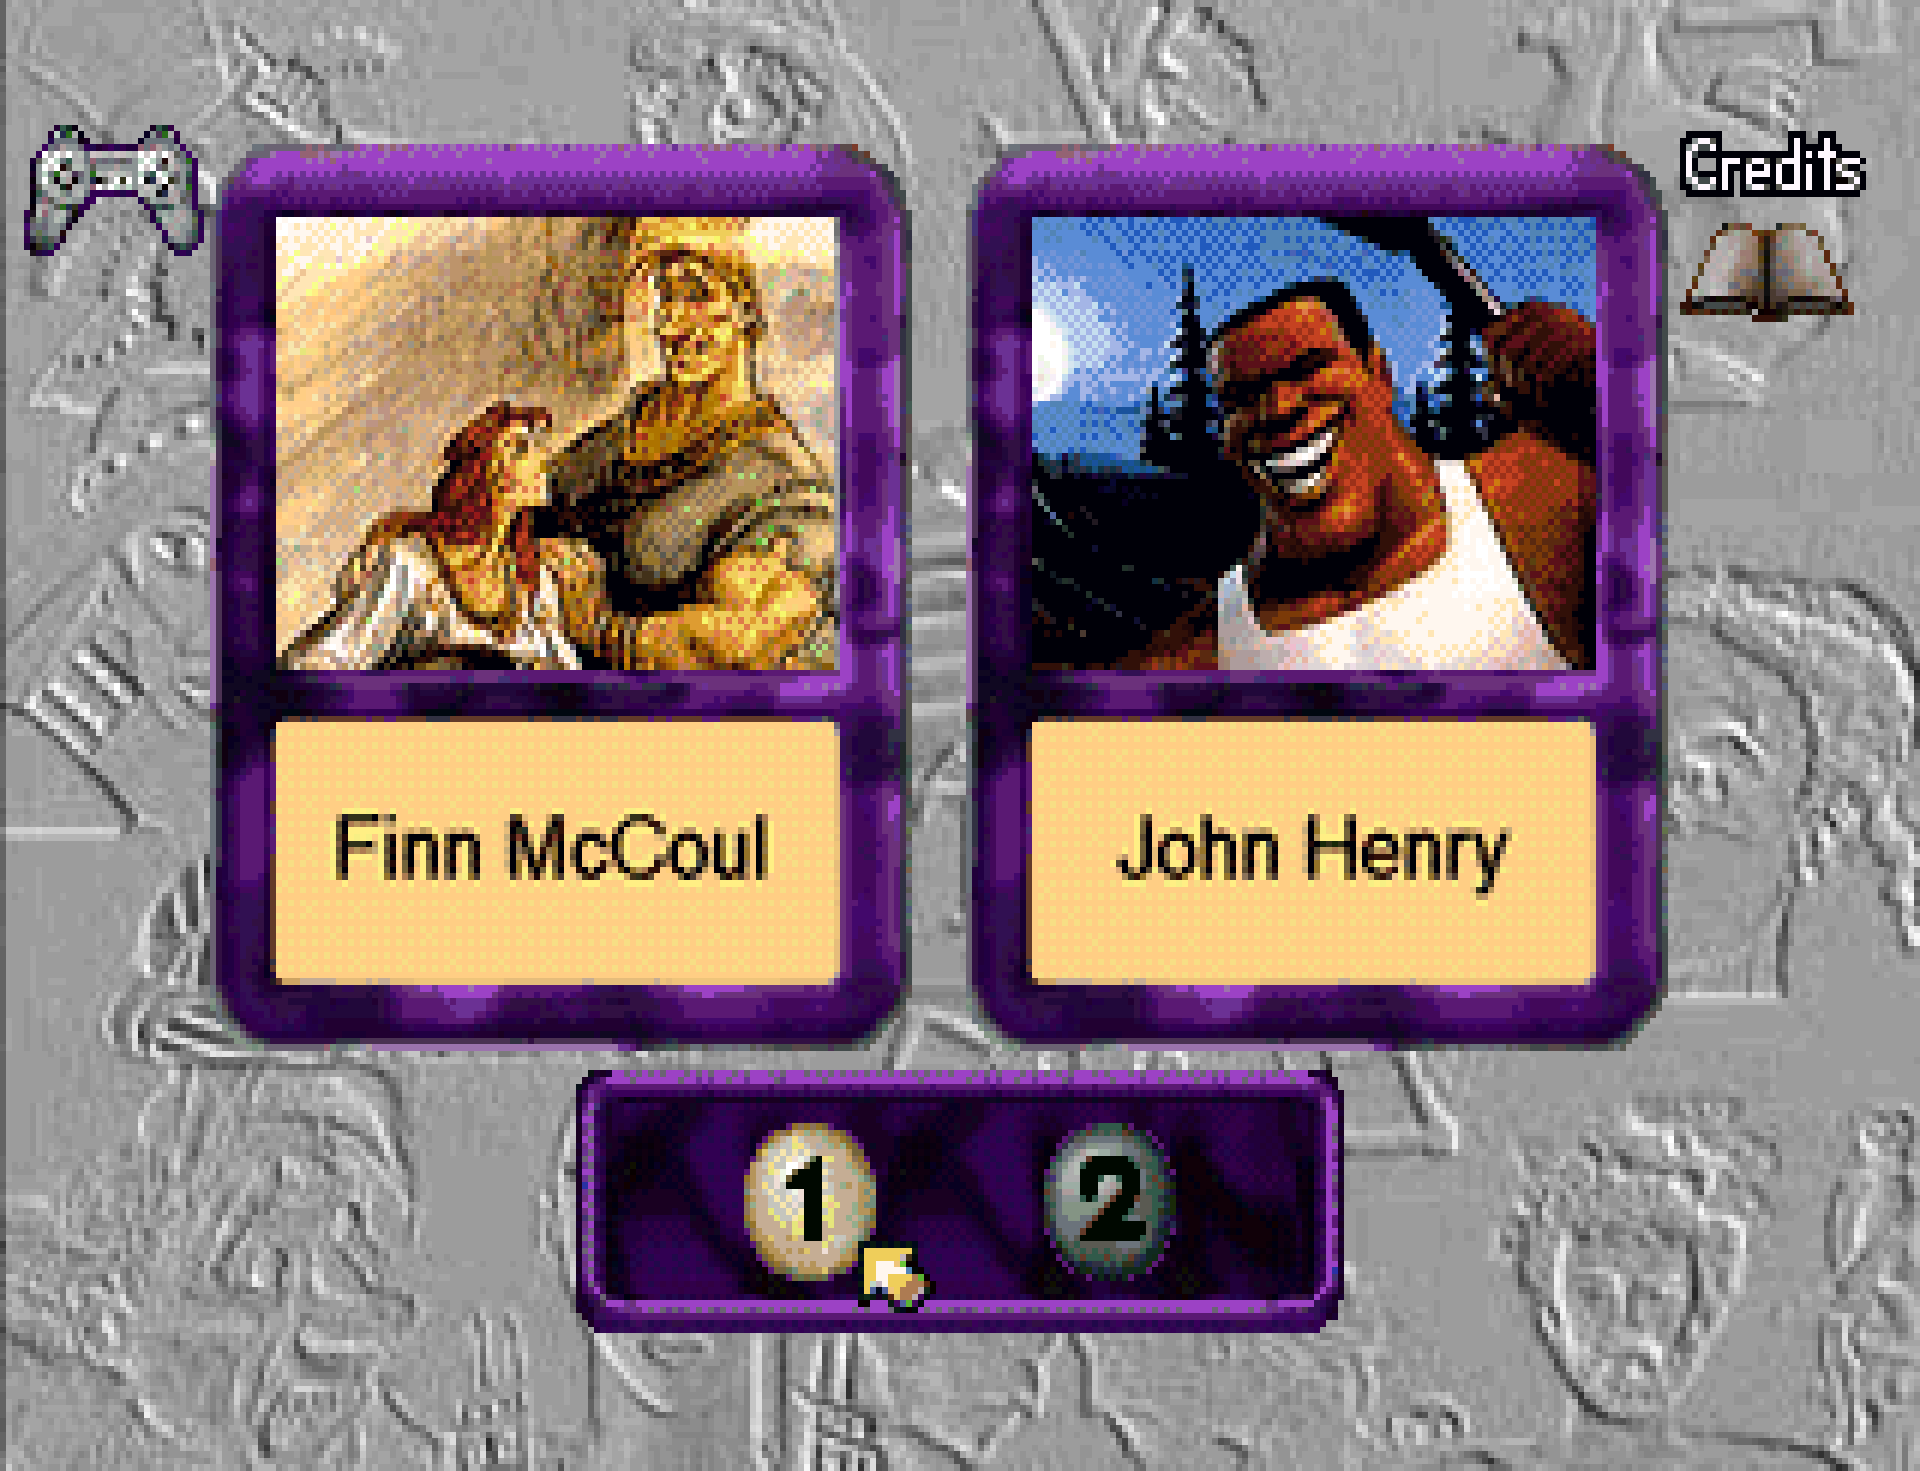
\includegraphics[width=\linewidth]{Games/StoryLaneTheater/Images/StoryLaneTheater2Image1.png}
        \caption{Story Lane Theater 2 - Screenshot 1}
    \end{subfigure}
    \begin{subfigure}{0.45\textwidth}
        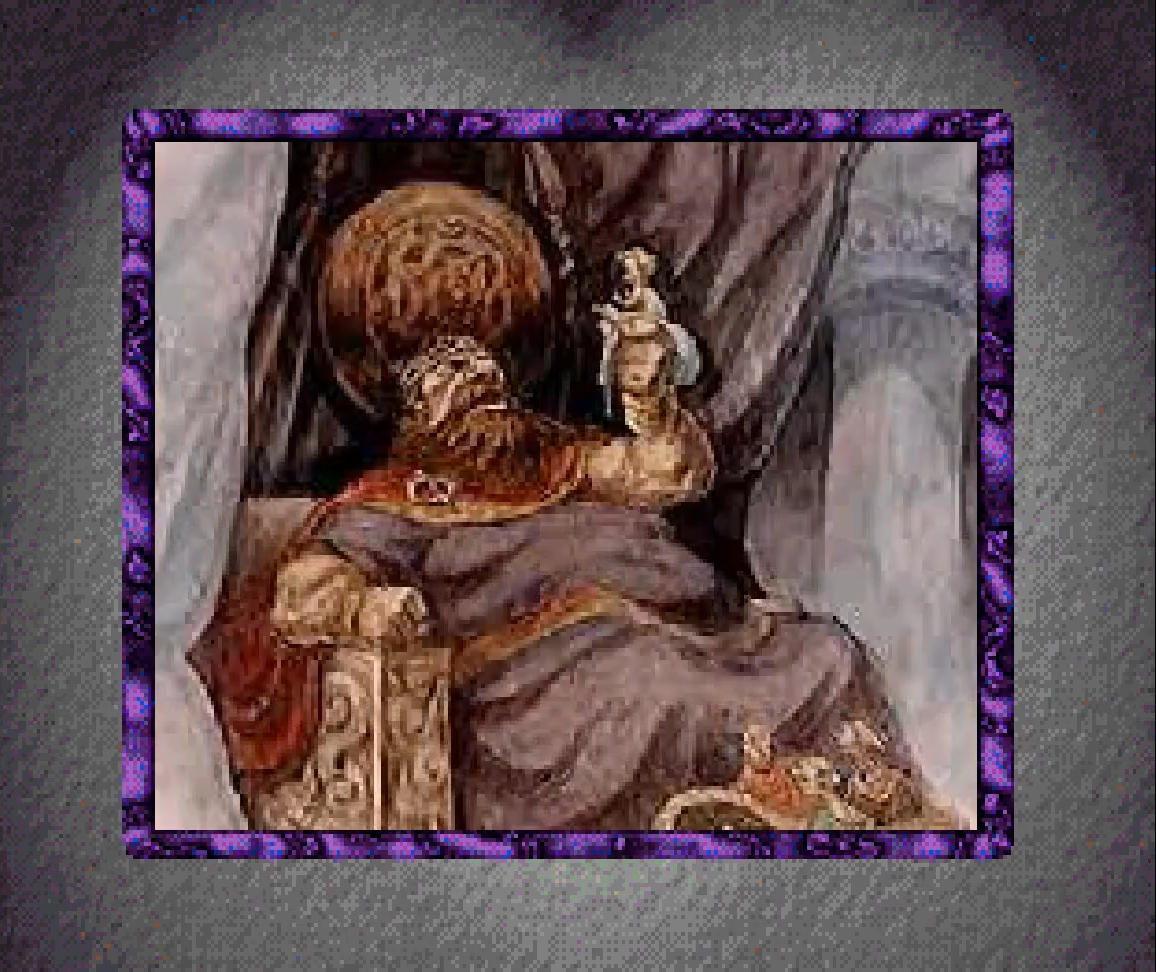
\includegraphics[width=\linewidth]{Games/StoryLaneTheater/Images/StoryLaneTheater2Image2.png}
        \caption{Story Lane Theater 2 - Screenshot 2}
    \end{subfigure}

    \begin{subfigure}{0.45\textwidth}
        \centering
        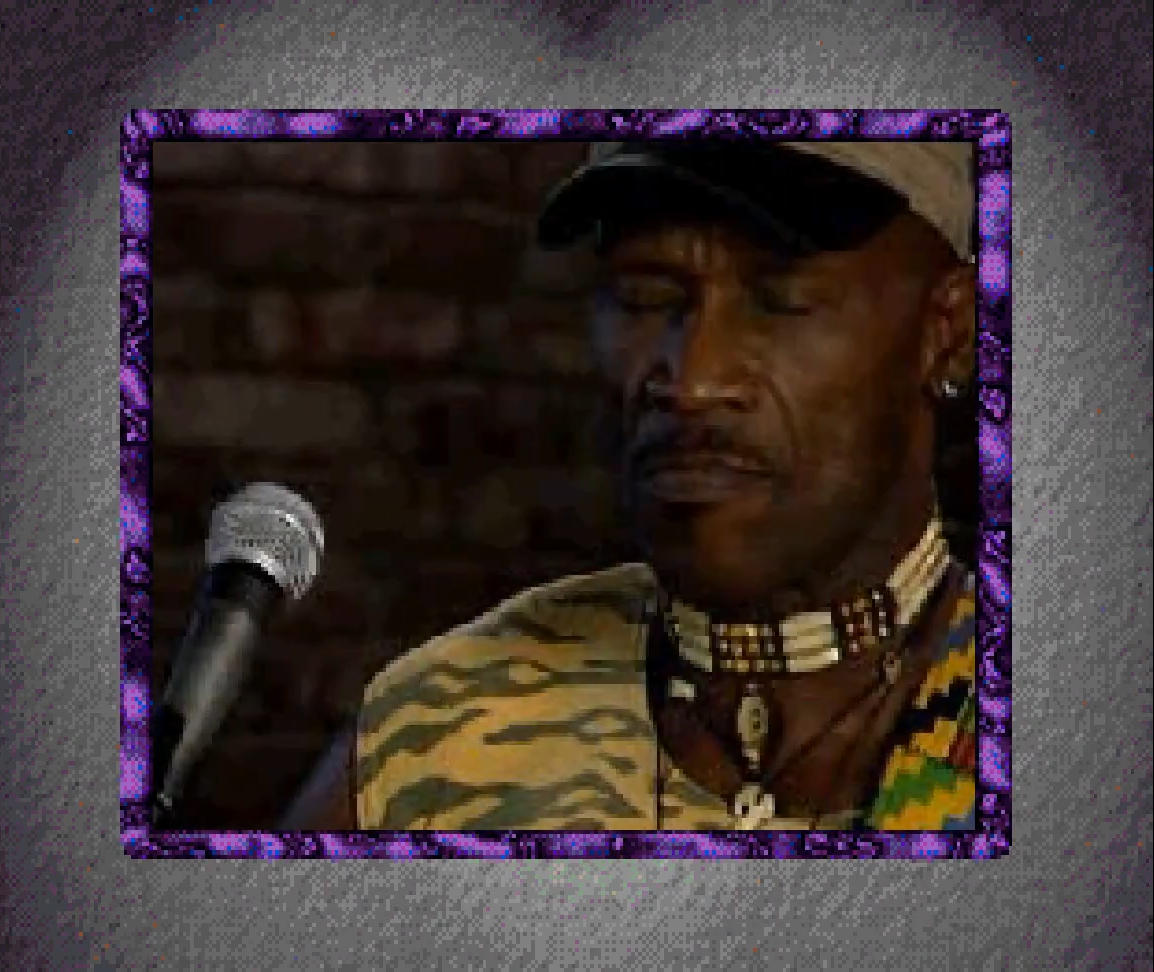
\includegraphics[width=\linewidth]{Games/StoryLaneTheater/Images/StoryLaneTheater2Image3.png}
        \caption{Story Lane Theater 2 - Screenshot 3}
    \end{subfigure}
    \begin{subfigure}{0.45\textwidth}
        \centering
        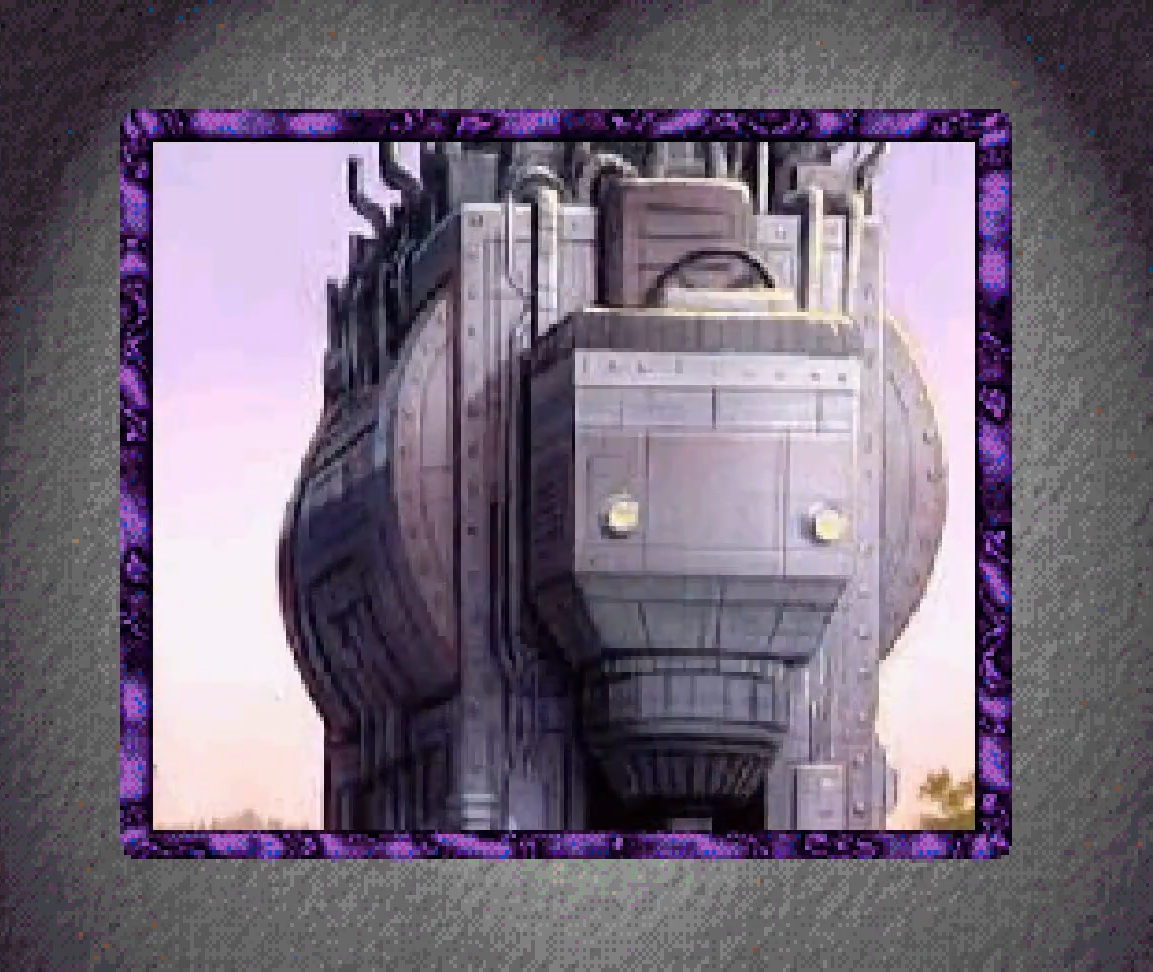
\includegraphics[width=\linewidth]{Games/StoryLaneTheater/Images/StoryLaneTheater2Image4.png}
        \caption{Story Lane Theater 2 - Screenshot 4}
    \end{subfigure}
    \caption{Screenshots from Story Lane Theater 2}
\end{figure}